\subsection{GBTL: GraphBLAS Template Library}
 
The first version of the GraphBLAS Template Library (GBTL) was written in C++ 
when the GraphBLAS C API project was just beginning.  It was used, in part, 
to study early ideas under discussion in the specification process and was released as a proof of concept 
prior to the finalization of the GraphBLAS API Specification \cite{gbtl-cuda16, McMillan2016}. With the 
release of the GraphBLAS C API Specification~\cite{cspec} in 2017, GBTL was updated to conform to 
the mathematical behavior defined by the specification and released as version 2.0~\cite{gbtl-github}.  
Unlike the C API Specification, GBTL is written in C++ and makes judicious use of templates to 
make the generic aspects of the GraphBLAS specification easier to implement and 
more natural for the C++ programming language. When the GraphBLAS language committee
starts its work on the C++ language binding to the GraphBLAS, GBTL will be submitted as a 
proposed starting point for the discussion.

 
As illustrated in Figure~\ref{fig:gbtl}, central to GBTL's design is the concept of a separation 
of concerns between implementation of algorithms written in terms of the GraphBLAS primitives 
and the implementation of those primitives on a targeted hardware platform.   Today the
 separation of concerns is defined by the GraphBLAS API Specification.  Above 
 this API, GBTL has developed and includes a collection of graph algorithms 
 written against its C++ API and has already been shown to be easily translated to the C API.  
 Below the separation/API, different implementations of the GraphBLAS library can be supported 
 for different hardware architectures (referred to as ``backends'').  In this way we verify that algorithms 
 written once against the API can run on different targeted hardware.  In terms of backend 
 implementations, a mathematically correct reference implementation (not optimized) for single 
 threaded CPU is provided with Version 2.0 of GBTL (version 1.0 also had a GPU implementation).  
 Other backend implementations are currently under development to target specialized computer architectures.

\begin{figure}[t]
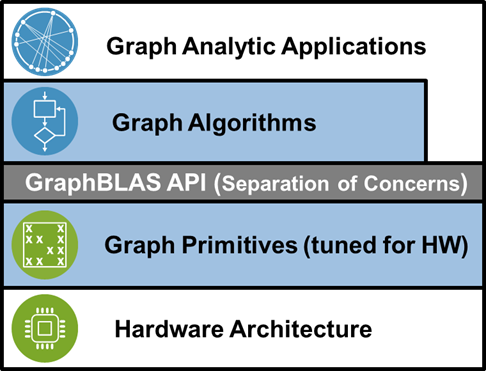
\includegraphics[width=\linewidth]{fig/gbtl}
\label{fig:gbtl}
\caption
{\textbf{Graph processing software stack.}}
\end{figure}
%
%  I don't know how to make the listing work below  so I will comment this out for now
%Another development effort closely related to GBTL is a DSL in python called pyGB~\cite{Chamberlin2016}.  
%The goal for pyGB is to closely resembles the GraphBLAS mathematical notation found in the GraphBLAS math spec~\cite{mathgraphblas16}.  
%PyGB is framework is designed and implemented to dispatch dynamically generated and compiled templated 
%classes that make calls into native GBTL code.  It demonstrates how Python's syntax and dynamic execution provides 
%a high-level abstraction with minimal performance penalty.  While we leave a detailed discussion of pyGB to elsewhere~\cite{Chamberlin2016}
%we provide a depth-BFS function using pyGB in figure~\ref{code:pyGB}.  Notice how the meaning of the code
%is straightforward since the DSL closely tracks the notation from the GraphBLAS math spec.  We believe in the long run, the 
%future of graph algorithms will depend heavily on such DSLs.
%
%\begin{CodeExample}
%{\textbf{Depth-BFS function in pyGB}}
%{code:pyGB}
%\begin{lstlisting}
%def bfs(graph, frontier, levels):
%    depth = 0
%    while frontier.nvals > 0:
%        depth += 1
%        levels[front][:] = depth
%        with gb.LogicalSemiring, gb.Replace:
%            frontier[~levels] = graph.T @ frontier 
%\end{lstlisting}
%\end{CodeExample}


